\documentclass[a4paper,12pt]{scrartcl}

\author{Matthew Cocci}
\title{Title}
\date{today}
\usepackage{enumitem} %Has to do with enumeration	
\usepackage{amsfonts}
\usepackage{amsmath}
\usepackage{amsthm} %allows for labeling of theorems
\usepackage[T1]{fontenc}
\usepackage[utf8]{inputenc}
\usepackage{blindtext}
\usepackage{graphicx}
%\numberwithin{equation}{section} 
%, This labels the equations in relation to the sections rather than other equations
%\numberwithin{equation}{subsection} %This labels relative to subsections
\newtheorem{thm}{Theorem}[section]
\newtheorem{lem}[thm]{Lemma}
\newtheorem{prop}[thm]{Proposition}
\newtheorem{cor}[thm]{Corollary}
\setkomafont{disposition}{\normalfont\bfseries}
\usepackage{appendix}


\begin{document}

\begin{center} \LARGE \bf
   The Multivariate Normal Distribution
\end{center}

The univariate normal distribution is an extremely familiar concept
where some random variable $X$ can take values along the real with 
probabilities that match the famouse bell-curve. Recall 
the probability density function of
   \[ f_Y(y) = \frac{1}{\sigma \sqrt{2\pi}} \; e^{-\frac{1}{2\sigma^2}
      (y - \mu)^2} \]
However, that's 
limited to only one dimension, and we would like to generalize to 
higher dimensions. In the next-simplest
2-dimensional case, we'd like a distribution
that actually looks like a bell---where potentional values can
range over the real plane, $\mathbb{R}$, where the density is
clustered around some mean before tapering off in all directions, 
as seen below.
\begin{figure}[h!]
   \centering
   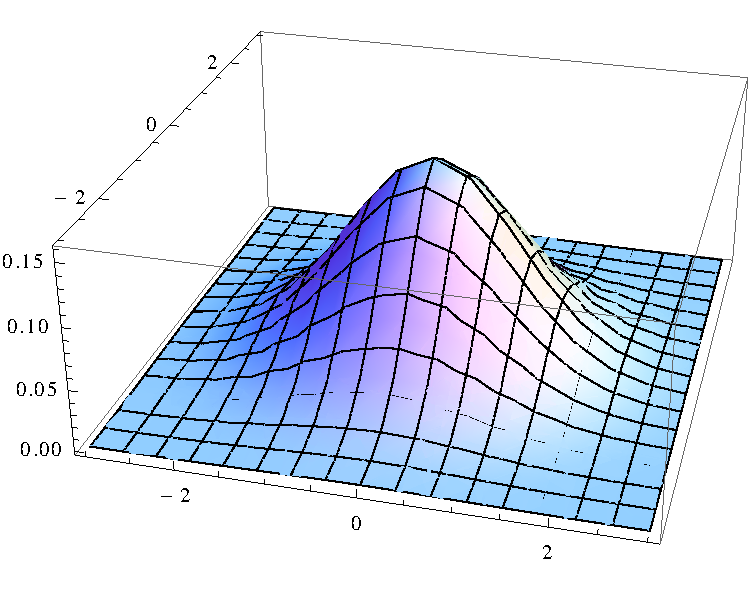
\includegraphics[scale=0.60]{multivariate.pdf}
\end{figure}
\\
This figure has mean zero for both $X_1$ and and $X_2$, and 
which are independent, implying $\sigma = I_2$, the identity matrix. 
It's easy to see that any vertical cuts parallel to $xz$ or $yz$ planes
will yield a traditional normal random variable. This of course 
generalizes to higher dimensions, although we can't display it so nicely.

\section{Notation}

In this note, the multivariate distribution will apply to a
$n$-dimensional random vector 
\[ \mathbf{X} = \begin{pmatrix} X_1 & X_2 & \ldots & X_n \end{pmatrix},
   \qquad \mathbf{X}  \sim N_n(\mu, \Sigma) \]
where $\mu$ is the $n$-dimensional \emph{mean vector},
\[ \mu = \begin{pmatrix} EX_1 & EX_2 & \ldots & EX_n \end{pmatrix},
      \]
and where $\Sigma$ is the $n\times n$ \emph{covariance matrix}, which
is defined and has in its $i,j$ entry
\[ \sigma = E\left[ (\mathbf{X} - \mu) (\mathbf{X}-\mu)'\right] \in
   \mathbb{R}^{N\times N} \] 
\[ \Sigma_{ij} = Cov(X_i, X_j), \qquad i,j = 1, \ldots, n\]

\section{Definition}

A random vector $\mathbf{X}$ has a \emph{multivariate normal} 
distribution if every linear combination of its components,
\[ Y = a_1 X_1 + \ldots + a_n X_n \] 
\[ \Leftrightarrow Y = \mathbf{a}' \mathbf{X}, \qquad
   \mathbf{a} \in \mathbb{R}^n \]
is \emph{normally
distributed}, with a corresponding mean and variance. This gives a 
joint density function of 
   \[ f_\mathbf{X}(\mathbf{x}) = \frac{1}{(2\pi)^{n/2} \lvert \Sigma
      \rvert^{1/2}} \; e^{ -\frac{1}{2} (\mathbf{x} - \mu)' \;
      \Sigma^{-1} (\mathbf{x} - \mu) }, \qquad \lvert\Sigma\rvert =
      \det\Sigma\]
   
\section{Joint Normality}

Suppose that $X$ and $Y$ are normally distributed and indepdent. This
then implies that they are \emph{jointly normally distrubed}. In other
words, $\begin{pmatrix} X & Y \end{pmatrix}$ must have a multivariate
normal distribution. Note, however, that $X$ and $Y$ must be independent 
for this to hold, not just uncorrelated.\footnote{Note that 
uncorrelated does not, in general, imply independence. Moreover, a lot
of confusions exist on this concept, so be very careful when considering
it.}






\end{document}

